\documentclass[a4paper]{article}
\usepackage{a4wide}
\usepackage[utf8]{inputenc}
\usepackage{amsmath}
\usepackage{mathtools}
\usepackage{amssymb}
\usepackage[english]{babel}
\usepackage{mdframed}
\usepackage{systeme,}
\usepackage{lipsum}
\usepackage{relsize}
\usepackage{caption}
\usepackage{tikz}
\usepackage{tikz-3dplot}
\usetikzlibrary{shapes.geometric}
\usepackage{pgfplots}
\usepackage{pgfplotstable}
\pgfplotsset{compat=newest}%1.7}
\usepackage{harpoon}%
\usepackage{graphicx}
\usepackage{wrapfig}
\usepackage{subcaption}
\usepackage{authblk}
\usepackage{float}
\usepackage{listings}
\usepackage{xcolor}
\usepackage{chngcntr}
\usepackage{amsthm}
\usepackage{comment}
\usepackage{commath}
\usepackage{hyperref}%Might remove, adds link to each reference
\usepackage{url}
\usepackage{calligra}

% Commands

\newcommand{\w}{\omega}
\newcommand{\F}{\mathcal{F}}
\newcommand{\curl}[1]{\mathbf{\nabla}\times \mathbf{#1}}
\newcommand{\grad}{\mathbf{\nabla}}
\newcommand{\dive}[1]{\mathbf{\nabla}\cdot \mathbf{#1}}
%\newcommand{\crr}{\mathfrak{r}}
\newcommand{\res}[2]{\text{Res}(#1,#2)}
\newcommand{\laplace}{\nabla^2}
\newcommand{\trace}{\text{Tr}}
\newcommand{\fpartial}[2]{\frac{\partial #1}{\partial #2}}
\newcommand{\rot}[3]{\begin{vmatrix}\hat{x}&\hat{y}&\hat{z}\\\partial_x&\partial_y&\partial_z\\#1&#2&#3 \end{vmatrix}}

% Special character commands
\DeclareMathAlphabet{\mathcalligra}{T1}{calligra}{m}{n}
\DeclareFontShape{T1}{calligra}{m}{n}{<->s*[2.2]callig15}{}
\newcommand{\crr}{\mathcalligra{r}\,}
\newcommand{\boldscriptr}{\pmb{\mathcalligra{r}}\,}



\title{Handin 4}
\author{Author : Andreas Evensen}
\date{Date: \today}
\definecolor{codegreen}{rgb}{0,0.6,0}
\definecolor{codegray}{rgb}{0.5,0.5,0.5}
\definecolor{codepurple}{rgb}{0.58,0,0.82}
\definecolor{backcolour}{rgb}{0.95,0.95,0.92}

\lstdefinestyle{mystyle}{
    backgroundcolor=\color{backcolour},   
    commentstyle=\color{codegreen},
    keywordstyle=\color{magenta},
    numberstyle=\tiny\color{codegray},
    stringstyle=\color{codepurple},
    basicstyle=\ttfamily\footnotesize,
    breakatwhitespace=false,         
    breaklines=true,                 
    captionpos=b,                    
    keepspaces=true,                 
    numbers=left,                    
    numbersep=5pt,                  
    showspaces=false,                
    showstringspaces=false,
    showtabs=false,                  
    tabsize=2
}

\lstset{style=mystyle}

\begin{document}

\maketitle

\section*{Exercise 1}
A bi-lipid layer is a two-dimensional fluid, in the sense that the shear elastic modulus $\mu$= 0.
The area modulus $K_A$ is not. Consider a vesicle of radius $R$ made out of bi-lipid layer. This sits on a rigid plate.
It is being poked by the tip of an atomic force microscope(AFM). Model the tip as a cone with opening angle $\alpha$. 
Assume that the volume of the vesicle remains unchanged. The change in bending energy is negligible.
Using the principle of virtual work (or any other-way) obtain the force-distance relationship for very small force. Hint: Consider the deformation to be localized.

\subsection*{Answer}
\begin{figure}[H]
    \centering
    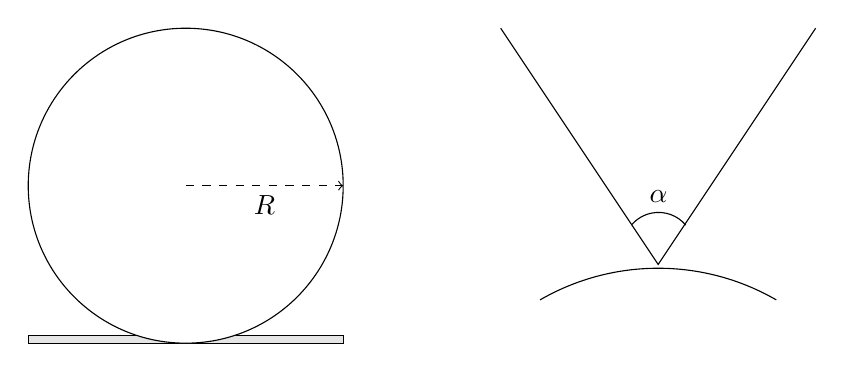
\begin{tikzpicture}
        % First
        \draw[fill = black!10] (0,0) rectangle (4,0.1);
        \draw[fill = white] (2,2) circle (2);
        \draw[->, dashed] (2,2) -- (4,2) node[pos = 0.5, below] {$R$};

        % Second
        \draw (6,5 - 1) -- (8, 2 - 1) -- (10, 5 - 1);
        \draw (9.5, 0.55) arc (60:90+30:3);
        \draw (8.35, 1.5) arc (40:140:0.45) node[pos = 0.5, above] {$\alpha$};
    \end{tikzpicture}
    \caption*{System layout}
\end{figure}\noindent
In the case, the bending of the vesicle is negligible, and thus we only consider two cases of deformation, namely stretching and area change. Since the bending is negligible, so is its contribution to the free energy.
Furthermore, since the stretching is dependent on the sheer-modulus $\mu$ so is its contribution to the free energy. Thus, we only consider the area change and the force pushing the vesicle down.
\begin{align*}
    \F &= \underbrace{\F_{bend} + \F_{stretch}}_{=0} + \F_{area} + F_{push}\\
    &= \F_{area} + \F_{push}
\end{align*}One minimizes the free energy, and get the following:
\begin{align*}
    0 &= \frac{\partial \F}{\partial \theta}\\
    &=
\end{align*}

\section*{Exercise 2, A tether pulling experiment}
Large (mircometer) sized vesicles made of bi-lipid layers are called GUV's -- Giant Unilamellar Vesicles. If a bead is brought close to it, the membrane gets attached to it.
If this bead is now pulled very slowly by an optical tweezer a thin cylindrical tube comes out of the vesicle as shown in a figure in the original paper. One assumes that $r<< L, R$.
Assume that the change in volume is negligible. First write its free energy. Assume its bending modulus is $B$. Divide the system into a sphere, a cylinder and a cylindrical cap. 
Write the bending energy for each part. Total bending energy is a sum of these three bending energies. Then calculate the contribution of stretching, area modulus is $K_A$.
Write the total free energy which contains contributions from bending, stretching and from the force pulling the tether.
As the tether is being pulled very slowly assume the system to be in equilibrium. The free energy should be a minimum. Show that the force is given by:
\begin{align*}
    F = 2\pi\sqrt{2B \tau}\quad \text{where} \quad \tau = K_A \left(\frac{a - a_0}{a_0}\right),
\end{align*}where $a$ is the area of the spherical and cylindrical part and $a_0$ is the area before the tether is pulled. The area of the cylindrical cap is ignored (why?). 
This remarkable result shows that the force is constant, independent of the length of the tether $L$. The result of the typical experiment shown in the original figure.
Be aware, that not every experiment of tether pulling gives this result.
\begin{figure}[H]
    \centering
    \includegraphics*[scale= 0.5]{figure2.png}
\end{figure}

\subsection*{Answer}
The free energy of the system is given by:
\begin{align*}
    \mathcal{F} &= \mathcal{F}_{bend} + \mathcal{F}_{pull} + \mathcal{F}_{stretch},\\
    \mathcal{F}_{bend} &= \mathcal{F}_{sphere} + \mathcal{F}_{cylinder} + \mathcal{F}_{cap},
\end{align*}where the components are given by:
\begin{comment}
\begin{align*}
    \mathcal{F}_{sphere} &= B\cdot\oint_{Sphere} \left(\frac{1}{R} - \frac{1}{L}\right)^2dx_1dx_2\\
    &= \frac{4\pi B}{2}\left(\frac{1}{R} - \frac{1}{L}\right)^2,\\
    \mathcal{F}_{cylinder} &= B\cdot\oint_{cylinder} \left(\frac{1}{R} - \frac{1}{L}\right)^2dx_1dx_2\\
    &=\frac{2\pi B}{L}\left(\frac{1}{R} - \frac{1}{L}\right)^2,\\
    \mathcal{F}_{cap} &= B\cdot\oint_{cap} \left(\frac{1}{R} - \frac{1}{L}\right)^2dx_1dx_2\\
    &=\frac{2\pi B}{R}\left(\frac{1}{R} - \frac{1}{L}\right)^2\\
    \implies \mathcal{F}_{bend} &= \frac{4\pi B}{2}\left(\frac{1}{R} - \frac{1}{L}\right)^2+\frac{2\pi B}{L}\left(\frac{1}{R} - \frac{1}{L}\right)^2 + \frac{2\pi B}{R}\left(\frac{1}{R} - \frac{1}{L}\right)^2
\end{align*}
\end{comment}
\begin{align*}
    \mathcal{F}_{sphere} &= B\cdot\oint_{Sphere} \left(\frac{1}{R} \right)^2dx_1dx_2\\
    %&= \frac{4\pi B}{2}\left(\frac{1}{R}\right)^2,\\
    \mathcal{F}_{cylinder} &= B\cdot\oint_{cylinder} \left(\frac{1}{r}\right)^2dx_1dx_2\\
    %&=\frac{2\pi B}{L}\left(\frac{1}{r}\right)^2,\\
    \mathcal{F}_{cap} &= B\cdot\oint_{cap} \left(\frac{1}{2r}\right)^2dx_1dx_2\\
    %&=\frac{2\pi B}{R}\left(\frac{1}{2r}\right)^2,\\
    \implies \mathcal{F}_{bend} &= B\left(\oint_{sphere}\left(\frac{1}{R}\right)^2dx_1dx_2+\oint_{cylinder}\left(\frac{1}{r}\right)^2dx_1dx_2 + \oint_{cap}\left(\frac{1}{2r}\right)^2dx_1dx_2\right).
\end{align*}The stretching energy is given by:
\begin{align*}
    \mathcal{F}_{stretch} &= \frac{K_A}{2}\oint\left(\frac{L}{L_0} - 1\right)^2dA,
\end{align*}The stretching energy is given by:
\begin{align*}
    \mathcal{F}_{pull} &= f\cdot L.
\end{align*}We now have the total free energy of the system, and moreover we know that the system is in equilibrium when the free energy is a minimum; and we assume it is in all instances.
\begin{align*}
    \frac{d\mathcal{F}}{df} &= 0 \\
    \implies& dF\cdot L + \frac{K_A}{2}\left(\frac{L}{L_0} - 1\right)^2 + B \left[\left(\frac{1}{R}\right)^2 + \left(\frac{1}{r}\right)^2 + \left(\frac{1}{2r}\right)^2\right] = 0.
\end{align*}


\section*{Exercise 3}
The figure 2 shows an AFM experiment on a (single walled) carbon nanotube rope.
This is a rope made of several single walled carbon nanotube. The data from the experiment is also given in the figure.
\begin{enumerate}
    \item Approximating the rope by an arc of a circle calculate a relationship between $F$ and $\delta$ following the treatment of a cantilever beam as done in class.  Assume bending is the only deformation.
    \item Assume the cross-section of the rope to be a circle of diameter $D$. If its' Young's modulus is $Y'$ first calculate its bending modulus. You can to integrate $$\int z^2 dzdy$$ over a circle of diameter $D$.
    \item From the data calculate $Y'$ and plot it against the diameter $D$. Now revisit our assumption of bending being only the deformation in the light of the data.
\end{enumerate}
The figure and the data are taken from the paper, Elastic and shear moduli of single-walled carbon nanotube ropes by J-P Salvetat, GADBriggs, J-M Bonard, RR Bacsa, AJ Kulik, Phys. Rev. Lett.,82, 944,(1999).2

\begin{figure}[H]
    \centering
    \includegraphics*[scale= 0.5]{figure1.png}
\end{figure}

\subsection*{Answer}
\subsection*{a}
\begin{figure}[H]
    \centering
    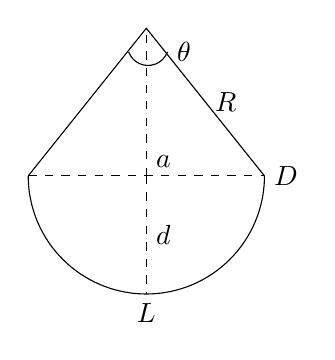
\begin{tikzpicture}[scale = 0.75]
        \draw[dashed] (-2,0) -- (2,0) node[right] {$D$};
        \draw (-2,0) arc (180:360:2) node[pos = 0.5, below] {$L$};
        \draw (-2,0) -- (0, 2.5) -- (2,0) node[pos = 0.5, right] {$R$};
        \draw[dashed](0,0) -- (0, 2.5) node[pos = 0.1, right] {$a$};
        \draw (-0.3, 2.1) arc (200:340:0.35) node[right] {$\theta$};
        \draw[dashed] (0,0) -- (0,-2) node[pos = 0.5, right] {$d$};
    \end{tikzpicture}
    \caption{Figure of the system}
\end{figure}\noindent
The figure above shows the system we're investigating. We assume that the rope is a circular arc of radius $R$, which then implies that the length of the rope $L$ is given by $L = R\theta$.
We also know that the displacement $d$ is given by $R - a$, and thus we need to find an expression for $a$. One make use of geometry to obtain the following:
\begin{align*}
    \cos\left(\frac{\theta}{2}\right) &= \frac{a}{R}\\
    \implies a &= R\cos\left(\frac{\theta}{2}\right),\\
    \implies d &= R - a = R\left(1 - \cos\left(\frac{\theta}{2}\right)\right)
\end{align*}We assume that only bending is the deformation, and the gravitational pull as well, and thus the free energy is given by:
\begin{align*}
    \mathcal{F} &= \frac{K}{2}\int_0^L\frac{1}{R^2}ds - F\cdot d\\
    &=\frac{KL}{2R^2} - F\cdot d =\frac{KL}{2R^2} - F\cdot R\left(1 - \cos\left(\frac{\theta}{2}\right)\right)\\
\end{align*}When the system is in equilibrium, the free energy is a minimum, and thus we have:
\begin{align*}
    \frac{d\mathcal{F}}{d\theta} &= 0\\
    \implies 0&= \frac{d}{d\theta}\left(\frac{K\theta^2}{2L} - F\cdot R\left(1 - \cos\left(\frac{\theta}{2}\right)\right)\right)\\
    &= \frac{K\theta}{L} - \frac{FL}{8}\\
    \implies d &= \frac{FL^3}{64K}.
\end{align*}

\subsection*{b}
We compute the following integral:
\begin{align*}
    I &= \oint_{circle} z^2 dydz\\
    &= \int_0^\pi\cos^2(\theta) d\theta\int_0^{\frac{D}{2}}r^2dr\\
    &=\frac{\pi}{4}\left(\frac{D}{2}\right)^4
\end{align*}We also know $K = Y\cdot I$ and thus $Y = \frac{K}{I}$. The expression for the Young's modulus is thus given by:
\begin{align*}
    Y &= \frac{K}{I}\\
    &= \left(\frac{FL^3}{64d}\right)\left(\frac{\pi D^4}{64}\right)^{-1}\\
    &= \frac{FL^3}{d\pi D^4}.
\end{align*}

\subsection*{c}
We're given a set of data points in the figure above. We use them to compute the Young's modulus, $Y$, against the diameter $D$.
\begin{figure}[H]
    \centering
    \begin{tikzpicture}
        \begin{axis}[
            xlabel = {$D$ $[a,u]$},
            ylabel = {$Y$ $[a.u]$},
            ymin = 0,
            ymax = 4000,
            xmin = 0,
            xmax = 20,
        ]
            \addplot+[blue] table {test.dat};
            \legend{$Y'_{comp}$.}
        \end{axis}
    \end{tikzpicture}
    \caption{Young's modulus plotted against the diameter of the rope.}
    \label{fig:task3c}
\end{figure}\noindent
As can be seen in the above figure, the Young's modulus is not constant but rather decreases with increasing diameter. This is not in accordance with our assumption that the only deformation is bending, in that case, the Young's modulus should be constant.
Here one sees a decaying behavior, $Y\propto e^{-D\lambda}$.

\end{document}
 